\chapter{Formal Analysis using Alloy}
This section provides a formal specification of the entire model using the Alloy language. We will use Alloy 6 to describe entities and relationships in systems. We choose Alloy 6 because is suited for modeling and analyzing the properties of software systems to ensure correctness and consistency.

\section{ Code}
\begin{lstlisting}
open util/relation
open util/boolean

//----SIGNATURES----
// User's role: it can be a student or a company
abstract sig Role {}
sig Student extends Role {
    applications: some Application
}
sig Company extends Role {
    postings: some Internship
}

// Users' personal information
sig User {
    email: one Email,
    otherInformation: one PersonalData,
    role: one Role
}
sig Email{}
sig PersonalData{}

// Internship
sig Internship {
    postedBy: one Company,
     applicants: some Application,
    description: one Description,
}
sig Description{}

// Application for an internship
sig Application {
    submittedBy: one Student,
    relatedTo: one Internship,
    interviews: one Interview,
    var status:  Status
}
enum Status {Pending, Accepted, Rejected}

// Interview
sig Interview {
    schedule: one DateTime,
    var outcome:  Outcome
}
enum Outcome {Passed, Failed, InProgress}
sig DateTime{}

//----FACTS----
// No two Users can have the same email or personal info
fact UniqueUsersEmailsAndPersonalInfo {
    all u1, u2: User | u1 != u2 implies
    u1.email != u2.email and
    u1.otherInformation != u2.otherInformation
}

// A role can only be associated with one User
fact OneUserPerStudentAndCompany{
    all s: Student | one u: User | u.role = s and
    all c: Company |  one u: User | u.role = c
}

//DoubleArrowConstraint
fact DoubleAssociation {
    //An interview can only be associated with an application
    all i: Interview | one a: Application | 
    i in a.interviews
   //An application can only be associated with a student
   all a: Application | one s: Student | 
   s in a.submittedBy and a in s.applications and
   s.applications.submittedBy=s
   //An application can only be associated with a Intenship
    all a: Application | one i: Internship | 
    a in i.applicants and  i in a.relatedTo and
    i.applicants.relatedTo = i
    //An internship can only be associated with a Company
    all  i:Internship | one c: Company | 
    c in i.postedBy and i in c.postings and 
    c.postings.postedBy = c  
}

// A student can make only an application for one internship
fact UniqueApplicationsPerStudent {
    all s: Student | all i: Internship | 
    #(s.applications & i.applicants) <= 1
}

// All applications are related to real posted Internship
fact ApplicationLinkedToValidInternship {
    all a: Application | a.relatedTo.postedBy in Company
}

//Two internships cannot have the same description 
fact UniqueInternshipsPerCompany {
    all i1, i2: Internship | i1 != i2 implies 
    i1.description != i2.description
}

//Two students cannot have the same application
fact UniqueApplicationsPerStudent {
    all s1,s2: Student | s1!=s2 implies 
    s1.applications != s2.applications
}

// All applications that are scheduled are applications that are really submitted by a student
fact InterviewApplicationRelation {
    all a: Application | a.interviews.schedule != none 
    implies a.submittedBy in Student
}

//A role cannot have a mettengs the same day
fact SameDayMeetings {
   all ss1,ss2: Student | all cc1,cc2: Company |
   all a1,a2: Application | a1!=a2 and
   ((ss1 in a1.submittedBy and ss2 in a2.submittedBy and
   cc1 in a1.relatedTo.postedBy and cc1 in a1.relatedTo.postedBy)or
  (ss1 in a1.submittedBy and ss1 in a2.submittedBy and
  cc1 in a1.relatedTo.postedBy and cc2 in a1.relatedTo.postedBy))
  implies a1.interviews.schedule != a2.interviews.schedule
}

fact InitialApplicationStatus {
    all a: Application | a.status = Pending
}
fact InitialInterviewOutcome {
    all i: Interview | i.outcome = InProgress
}

\end{lstlisting}



\section{ Models}
\subsection{Static Analysis}
\textbf{[MS1]} The model shows the basic scenario where one student is applying for an internship at a company with pending status and an in-progress interview.
\begin{lstlisting}
run {} for 2 but exactly 1 Student, exactly 1 Company, exactly 1  Internship
\end{lstlisting}
\begin{figure}[H]
    \centering
    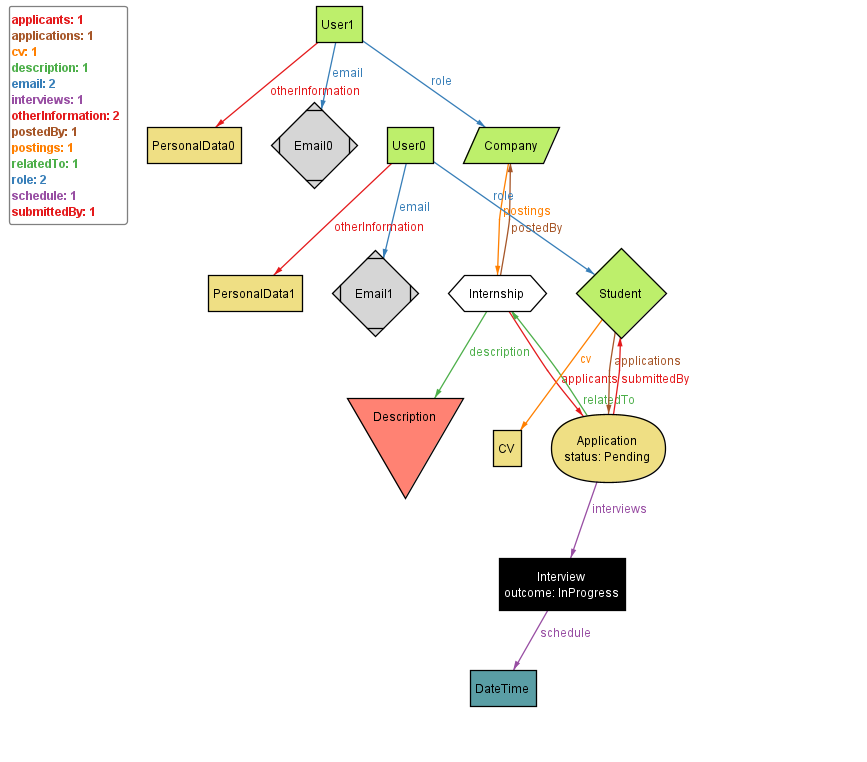
\includegraphics[width=0.75\linewidth]{RASD//Images/1st1com.png}
    \caption{1 Student, 1 Company, 1 Internship}
    \label{fig:enter-label}
\end{figure}

\textbf{[MS1]} The model shows a scenario where two students are applying for an internship at a company with pending status and an in-progress interview.
\begin{lstlisting}
run {} for 3 but exactly 2 Student, exactly 1 Company, exactly 1  Internship
\end{lstlisting}
\begin{figure}[H]
    \centering
    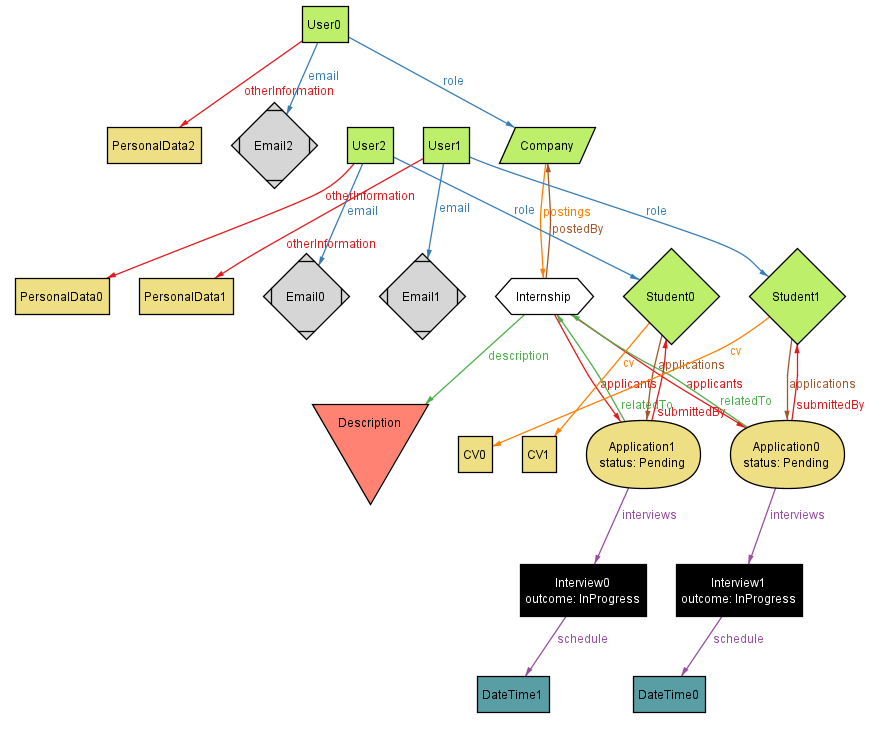
\includegraphics[width=0.75\linewidth]{RASD//Images/2st1com.png}
    \caption{2 Student, 1 Company, 1 Internship}
    \label{fig:enter-label}
\end{figure}

\textbf{[MS3]} The model shows a scenario where one student is applying for three internships 2 at company A and one at company B with pending status and an in-progress interview.
\begin{lstlisting}
run {} for 3 but exactly 1 Student, exactly 1 Company, exactly 3 Application
\end{lstlisting}
\begin{figure}[H]
    \centering
    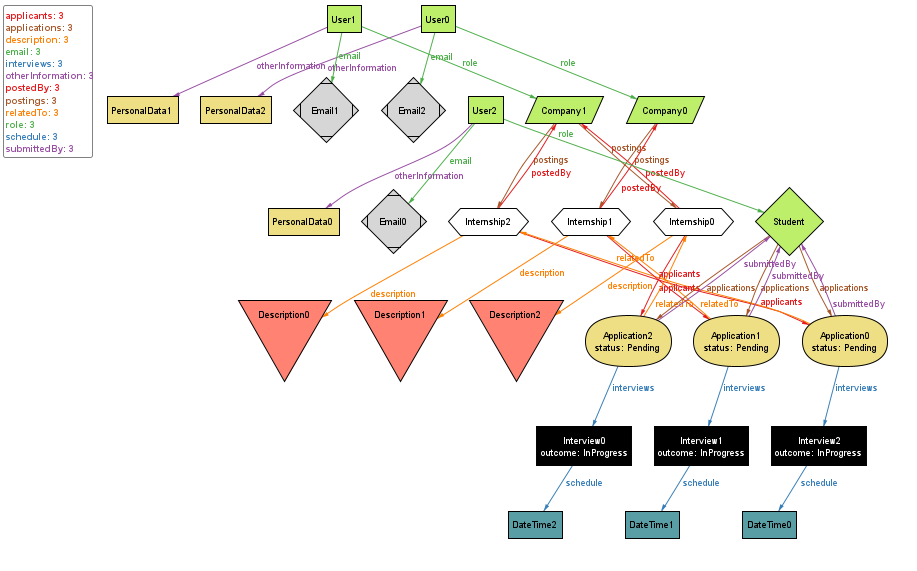
\includegraphics[width=0.75\linewidth]{RASD//Images/1st2com.png}
    \caption{1 Student, 1 Company, 3 Application}
    \label{fig:enter-label}
\end{figure}

\subsection{Dynamic Analysis}
\textbf{[MD1]}

\section{ Assertions}
\textbf{[A1]} Assertion to verify the correctness of the user structure as:
\begin{itemize}
    \item No Users will have the same email or the Personal info
    \item Each role can only be associated with one User
\end{itemize}
\begin{lstlisting}
//Assertion to verify the correctness of the user structure as:
assert VerifyUserStructure{
    all u1, u2: User | u1 != u2 implies 
    u1.email != u2.email and  u1.otherInformation != u2.otherInformation
    all s: Student | one u: User | u.role = s
    all c: Company | one u: User | u.role = c
}
check VerifyUserStructure
\end{lstlisting}
\textit{\#1: VerifyUserStructure may be valid.}

\textbf{[A2]} Assertion to verify DoubleArrowConstraint:
\begin{itemize}
    \item An interview can only be associated with an application
    \item An application can only be associated with a student
    \item An application can only be associated with a Intenship
    \item An internship can only be associated with a Company
\end{itemize}
\begin{lstlisting}
//Assertion to verify DoubleArrowConstraint
assert VerifyDoubleAssociation {
    all i: Interview | one a: Application | 
    i in a.interviews
    all a: Application | one s: Student | 
    s in a.submittedBy and a in s.applications and
    s.applications.submittedBy=s
    all a: Application | one i: Internship | 
    a in i.applicants and  i in a.relatedTo and
    i.applicants.relatedTo = i
    all  i:Internship | one c: Company | 
    c in i.postedBy and i in c.postings and 
    c.postings.postedBy = c  
}
check VerifyDoubleAssociation
\end{lstlisting}
\textit{\#2: VerifyDoubleAssociation may be valid.}

\textbf{[A3]} Assertion to verify all Internship application structure
\begin{itemize}
    \item Students can make only one application for each internship
    \item All applications are related to valid posted internships
    \item A company can't publish two equal internships 
    \item All scheduled interviews are actually submitted
    \item Two students cannot have the same application
    \item meetings company side
\end{itemize}
\begin{lstlisting}
// Assertion to verify all Internship application structure
assert VerifyInternshipStructures {
    all s: Student | all i: Internship | 
    #(s.applications & i.applicants) <= 1
    all a: Application | a.relatedTo.postedBy in Company
    all i1, i2: Internship | i1 != i2 implies i1.description != i2.description
    all a: Application | a.interviews.schedule != none implies a.submittedBy in Student
    all s1,s2: Student | s1!=s2 implies s1.applications != s2.applications
    all ss1,ss2: Student | all cc1,cc2: Company |
    all a1,a2: Application | a1!=a2 and
   ((ss1 in a1.submittedBy and ss2 in a2.submittedBy and
    cc1 in a1.relatedTo.postedBy and cc1 in a1.relatedTo.postedBy)or
   (ss1 in a1.submittedBy and ss1 in a2.submittedBy and
   cc1 in a1.relatedTo.postedBy and cc2 in a1.relatedTo.postedBy))
   implies a1.interviews.schedule != a2.interviews.schedule
}
check VerifyInternshipStructures
\end{lstlisting}
\textit{\#3: VerifyInternshipStructures may be valid}
